\section{Results}\label{sec:results}
%======================================================================

\subsection{Geometry-to-transport backbone}

The results in this section are best read as a chain rather than as a bag of summary plots.  They correspond to the exact-characteristic reference chain discussed earlier, not to every current canonical backend equally.  In the current code base, the same figures should be understood as reference-path results reproduced by matched exact-characteristic JAX surfaces and contextualised relative to the broader JAX-first default envelope.

The geometry figure in \S\ref{sec:geometry} illustrates the first step of that historical diagnostic chain: a time-dependent interaction between the shear, the Hubble enhancement, and the neutrino anisotropic stress.  The next step is the transport-to-weak bridge.  The characteristic rays accumulate a direction-dependent energy shift, and the diagnostic monopole is obtained by ray quadrature rather than by a momentum-independent linearised closure.  These plots predate the publication programme's B-03/B-05 validation and are not current finite-shear evidence.

\begin{figure*}[t]
\centering
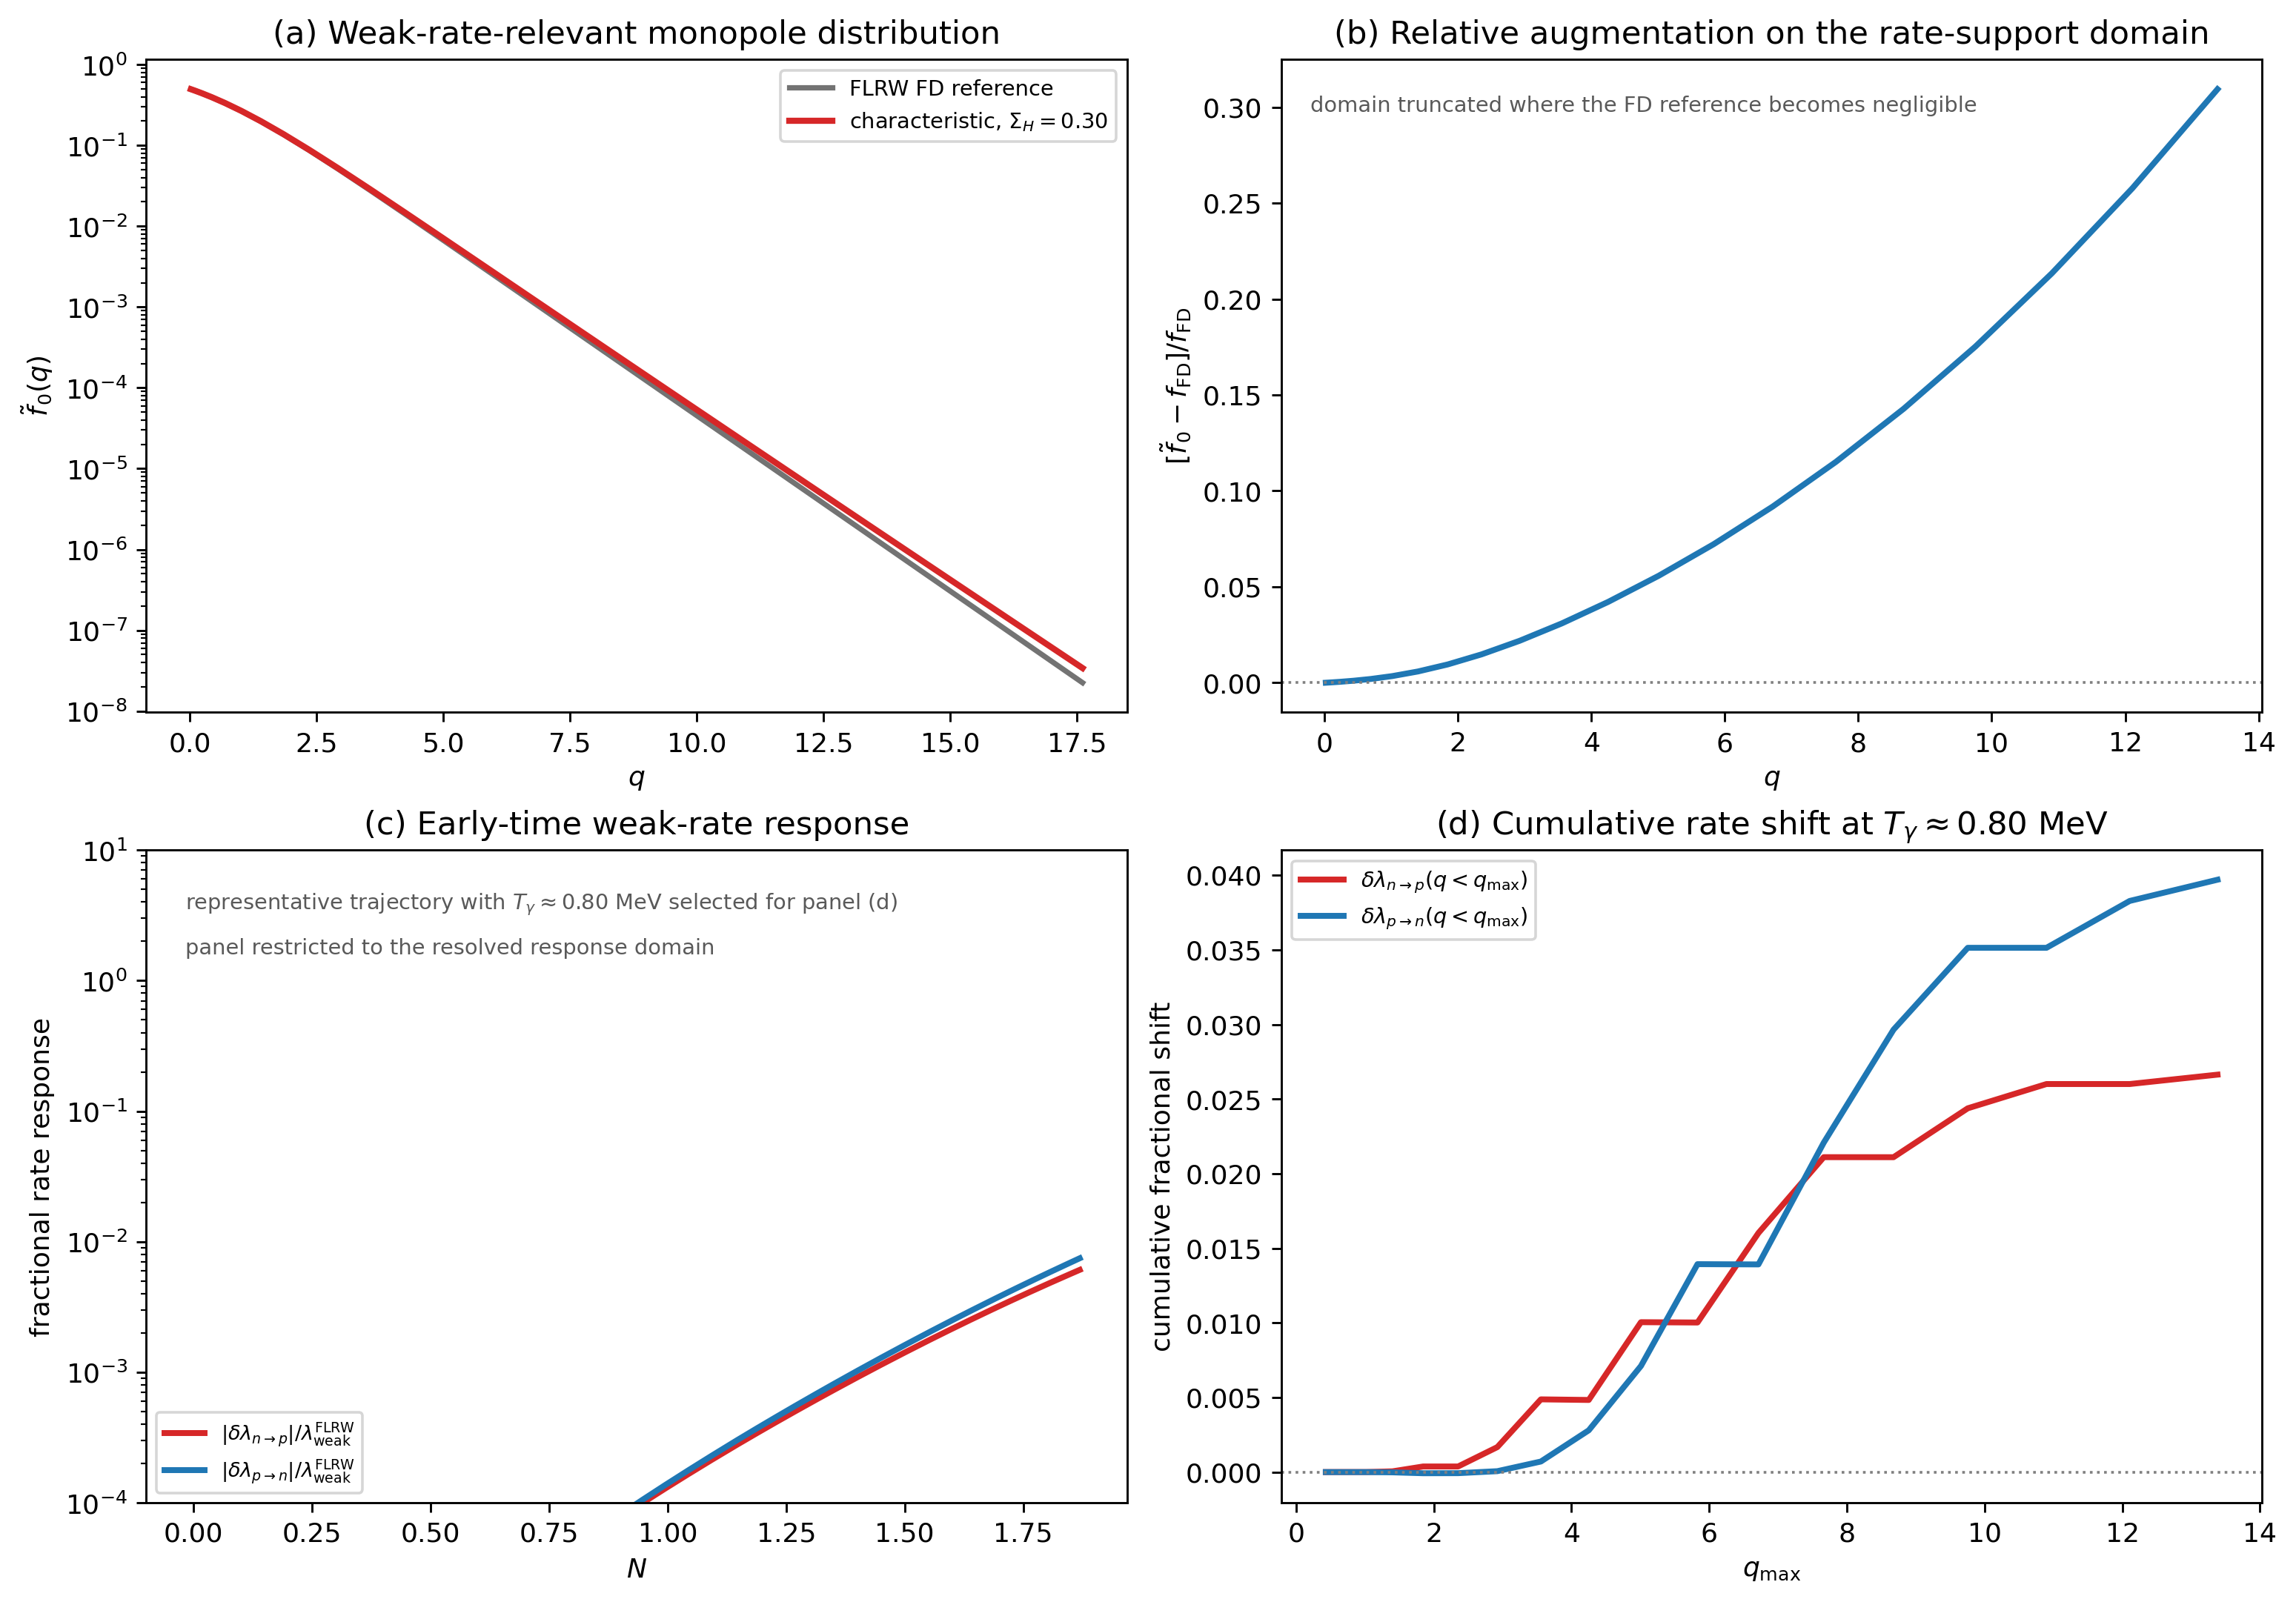
\includegraphics[width=\textwidth]{figures/fig_story_distribution_weak_bridge.png}
\caption{Bridge from the augmented monopole to the weak rates.  (a) The characteristic solution produces a weak-rate-relevant monopole $\tilde f_0(q)$ that is harder than the FLRW Fermi--Dirac reference.  (b) The relative augmentation grows toward the high-$q$ rate-support domain.  (c) The resulting perturbation induces a finite weak-rate response on the resolved early-time domain relevant for freeze-out.  (d) Integrating over momentum shows a cumulative fractional shift in $\lambda_{n\to p}$ and $\lambda_{p\to n}$ at the representative epoch $T_\gamma \simeq 0.80$ MeV.  Together these panels exhibit the middle link between characteristic transport and the final BBN-yield shift.}
\label{fig:story_bridge}
\end{figure*}

The central lesson of Fig.~\ref{fig:story_bridge} is that the characteristic method matters not merely because it produces a different quadrupole, but because it changes the weak-rate-relevant monopole itself.  The distortion is small at low momentum and grows across the rate-support domain, so the weak kernels are probed by a harder spectrum than the FLRW reference.  That is the physically important middle link between anisotropic transport and the observable BBN response.

\subsection{Direct BBN yield response}

\begin{table}[t]
\centering
\caption{BBN yields vs $\Sigma_H$ (CL2, characteristic transport, $\eta = 6.104 \times 10^{-10}$, $\tau_n = 878.4\,\mathrm{s}$).}\label{tab:yields}
\begin{tabular}{ccccc}
\toprule
$\Sigma_H$ & $\Yp$ (char) & $\Yp$ (lin) & $\Delta\Yp^{\rm NL}$ & D/H $\times 10^5$ \\
\midrule
0    & 0.24803 & 0.24803 & ---                   & 2.520 \\
0.10 & 0.24817 & 0.24807 & $+9.8\times 10^{-5}$  & 2.521 \\
0.30 & 0.24926 & 0.24839 & $+8.7\times 10^{-4}$  & 2.528 \\
0.50 & 0.25126 & 0.24917 & $+2.1\times 10^{-3}$  & 2.541 \\
\bottomrule
\end{tabular}
\end{table}

The resulting yield response is monotonic in $\Sigma_H$: increasing anisotropy raises $\Yp$ and, more weakly, D/H.  The nonlinear correction $\Delta\Yp^{\rm NL}$ grows super-linearly because the momentum-dependent spectral remapping is itself nonlinear in the accumulated characteristic energy shift.

\begin{figure*}[t]
\centering

\includegraphics[width=\textwidth]{figures/fig18.png}
\caption{Historical diagnostic BBN response to anisotropic expansion.  The panels show legacy CL2 outputs for $Y_p$ and D/H as functions of $\Sigma_H$, together with observational bands and the FLRW reference.  The dashed vertical line is a legacy runtime guard, not a validated physical-domain boundary.  The figure does not establish a publication constraint; B-03 and B-05 remain open.}
\label{fig:observable_response}
\end{figure*}

\subsection{Historical profile-likelihood diagnostic (not validated)}

Using $\Yp^{\rm obs} = 0.2449 \pm 0.0040$ (Aver et al.) and $(\mathrm{D/H})^{\rm obs} = (2.547 \pm 0.029) \times 10^{-5}$ (Cooke et al.), the legacy Type~I CL2 grid emitted a numerical crossing near $\Sigma_H=0.66$.  That value is a \textbf{DEPRECATED diagnostic readout}, not a validated confidence bound, and must not be cited as a current science result.  A finite-shear domain and canonical likelihood are not validated until B-03 and B-05 pass.

\begin{figure*}[t]
\centering
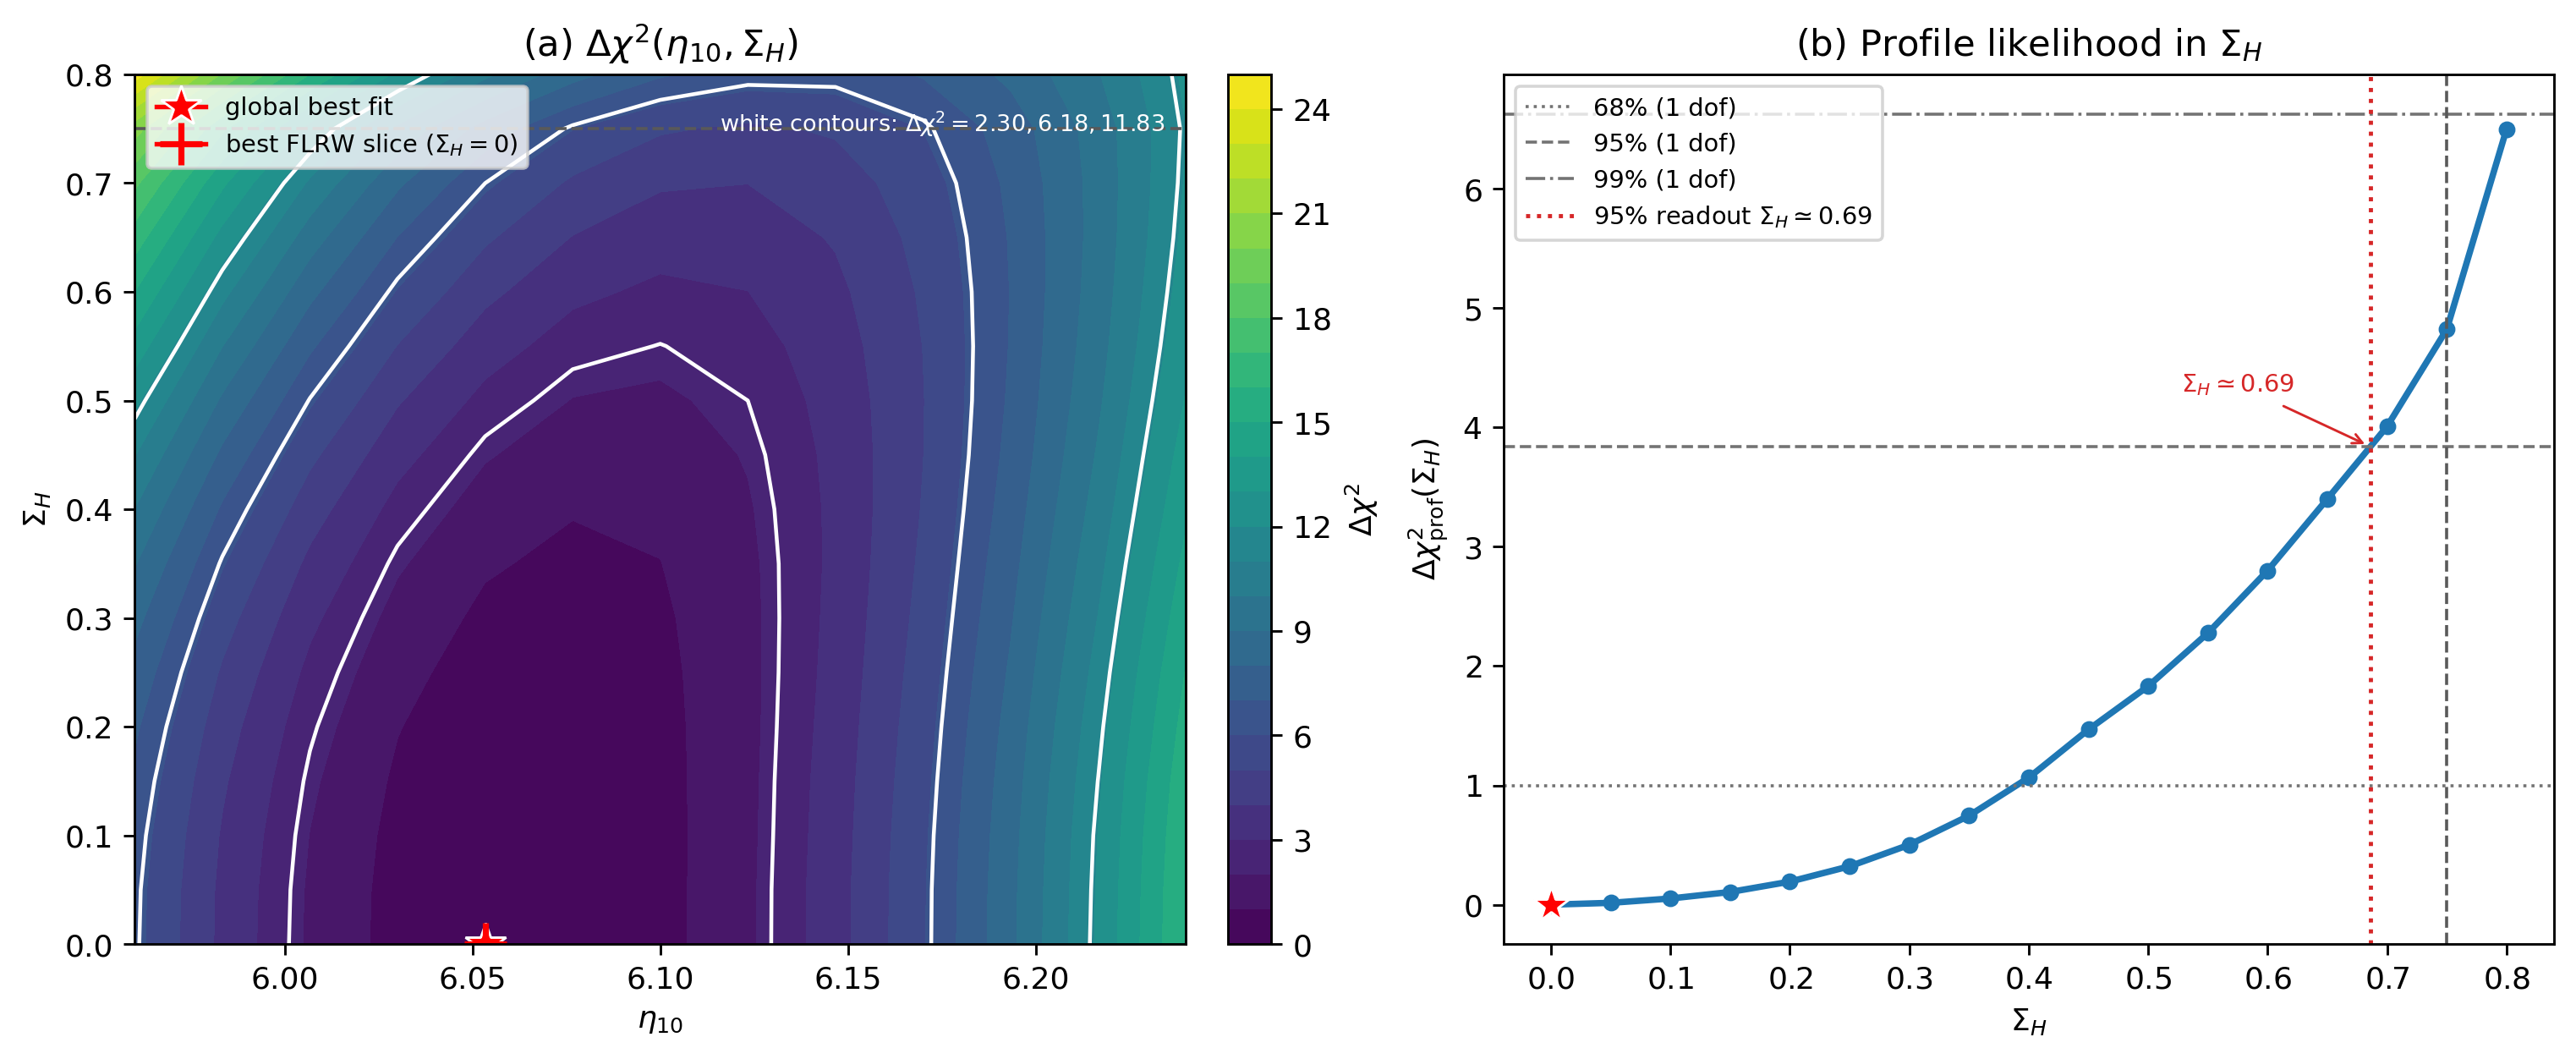
\includegraphics[width=\textwidth]{figures/fig21.png}
\caption{Historical diagnostic likelihood structure for the legacy Type~I grid.  Panel~(a) shows $\Delta\chi^2(\eta_{10},\Sigma_H)$ and reference contour levels; panel~(b) shows the corresponding profile statistic.  Neither the $0.75$ runtime guard nor the crossing is a validated publication domain or constraint.}
\label{fig:chi2}
\end{figure*}

At Born level the legacy FLRW baseline lay slightly low in $\Yp$, while Coulomb and Sirlin corrections shifted that diagnostic comparison.  No preference or bound from this scan is promoted by the current publication programme; the canonical inference path is deferred to B-05.

%======================================================================
